\documentclass[11pt]{article}
\usepackage[T1]{fontenc}
\usepackage[utf8]{inputenc}
\usepackage[french]{babel}
\usepackage[a4paper]{geometry}
\usepackage{color}
\usepackage{changepage}
\usepackage{float}
\usepackage{amsmath}
\usepackage[hidelinks]{hyperref}
\usepackage{graphicx}
\usepackage{array}


\begin{document}
\begin{figure}
    
\includegraphics[height=1cm]{logolemansU.png}
    \hfill
    
\includegraphics[height=1cm]{logo_IC2.png}
\end{figure}
    \title { 
        \textcolor{blue}{Le Mans Université} \\
        \texttt{Licence Informatique 2ème année} \\
        \texttt{Module 174UP02 Rapport de projet}\\
        \textbf{Titre du projet}\\
        \href{https://github.com/Herebios/projet}{Lien vers le Github}
    }
    
    \author{Baptiste M, Lucas R, Nathan M, Ilann T} 
    \date{\today} 
    \maketitle

    \newpage
    \tableofcontents
    \newpage
    
    \section{Introduction}
    Nous sommes un groupe de quatre étudiants à l’université du Mans. Notre objectif à été de créer un jeu en respectant un délai d'environ 3 mois.
    Lors de notre phase de réflexion sur le jeu, nous souhaitions créer un jeu multijoueur en deux dimensions à l'aide de la librairie graphique SDL2 en langage C. 
    Lors d’une partie de notre jeu, deux équipes s'affrontent pour détruire la base adverse tout en protégeant la sienne. 
    Nous nous sommes fixé comme contrainte de développer ce jeu en réseau.

    \section{Conception}
    Dans le menu, chaque joueur choisit son pseudo et la classe de son personnage, lui conférant des capacités uniques qu’il peut utiliser au cours de la partie pour 
    prendre l’avantage sur l’équipe adverse. Dans le menu, vous avez le choix entre être le serveur de la partie, être joueur d’une partie ou être les deux à la fois. \\
    Après cela, vous arrivez dans une salle d’attente pour que les autres joueurs se joignent à vous. Une fois que la personne servant de serveur lance la partie, 
    le jeu se lance et il n’est plus possible de rejoindre la partie, même si vous étiez dedans, que vous quittez le jeu et que vous tentez de vous reconnecter. \\
    La map de notre jeu se décompose en plusieurs parties que nous appelons tuiles, chacune ayant un biome(neige, plaine, etc) choisi aléatoirement. \\
    Les joueurs ne peuvent visualiser qu’une tuile du jeu à la fois. Cependant, il est possible de changer de tuile en passant par des portes placées à différents endroits 
    aux bords de la tuile à la manière de \href{https://en.wikipedia.org/wiki/The_Binding_of_Isaac_(video_game)}{The Binding of Isaac}. \\
    Des obstacles sont générés aléatoirement sur la map, limitant les déplacements du joueur. \\
    Des monstres sont également présents sur la map, se dirigeant vers le joueur le plus proche pour l’attaquer. Lorsque le monstre est tué il lache un objet que le joueur peut
    rammaser et ajouter à son inventaire.\\
    Chaque objet a une rareté et confère au joueur différents effets. Plus la rareté de l’objet est élevée, plus les effets bonus conférés au joueur sont importants. \\
    Un système de combat est mis en place entre les joueurs d’équipes différentes lorsqu’ils se situent sur la même tuile. 
    Les points de vie ainsi que les objets du joueur sont affichés sur son écran à la manière d’un inventaire \href{https://fr.wikipedia.org/wiki/Minecraft}{Minecraft}.\\ 
    La gestion des entités dynamiques et des tuiles de la map sont gérées grâce à l’implémentation d’une liste générique. 
    Le serveur communique avec les clients en envoyant toutes les informations nécessaires à l’affichage du jeu par le client qui renvoie des informations au serveur 
    en fonction des changements opérés par le joueur. Les communications entre le serveur et le client sont effectuées via une file générique mise en place à cet effet.
    
    \section{Organisation du Projet}
        \subsection{Planning Prévisionnel}
        Ci-dessous notre planning prévisionnel sur 3 mois. (Voir Figure~\ref{fig:Gant})
        \begin{figure}[H]
            \begin{center}
                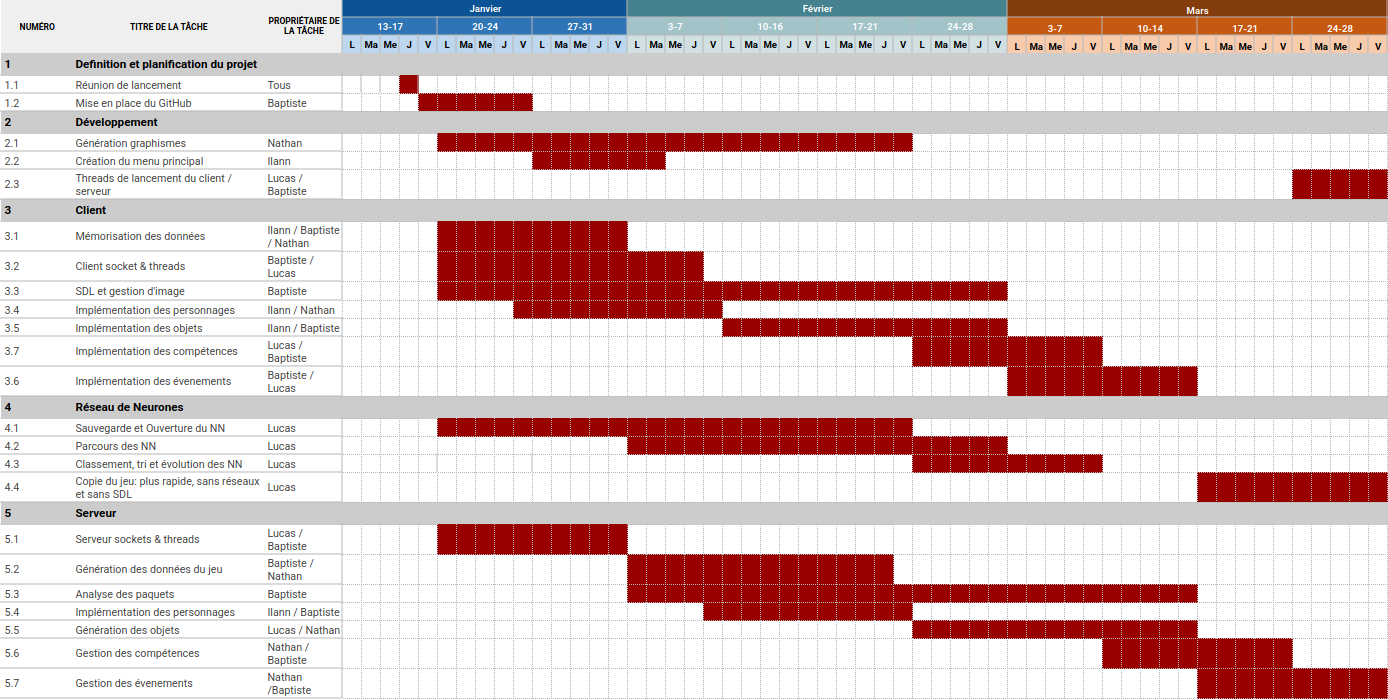
\includegraphics[height=9cm]{gant.png}
                \caption{Diagramme Gant}
                \label{fig:Gant} 
            \end{center}
        \end{figure}
        \subsection{Répartition des tâches}
        Nous nous sommes répartis les tâches de la manière suivante (se référer au numérotage sur le diagrame Gant Figure~\ref{fig:Gant}) :
        \begin{itemize}
            \item Baptiste : 1.1, 1.2, 3.1, 3.2, 3.3, 3.4, 5.1, 5.2, 5.4, 5.5
            \item Lucas : 1.1, 3.2, 4.1, 4.2, 4.3, 4.4, 5.1, 5.5
            \item Ilann : 1.1, 2.2, 3.1, 5.4
            \item Nathan : 1.1, 2.1, 3.1, 5.2, 5.5
        \end{itemize}
    \section{Développement}
    Cette partie abordera le développement du jeu dans sa globalité. De la création des ressources graphiques à la création du client/serveur en passant par la gestion des de la carte, des objets etc. 
        \subsection{Création des ressources}
        Cette section abordera la génération des ressources graphiques de base permettant la réalisation du jeu.
            \subsubsection{Objet}
            Il y a quarante objets dans le jeu. Tous générés avec un prompt chat gpt.\\
            Quelques exemples d'objets ci-dessous (Figure~\ref{fig:BagueMageNoir}, Figure~\ref{fig:OrbeMystique}).
            \begin{figure}[H]
                \centering
                % Première image
                \begin{minipage}{0.45\textwidth}
                    \centering
                    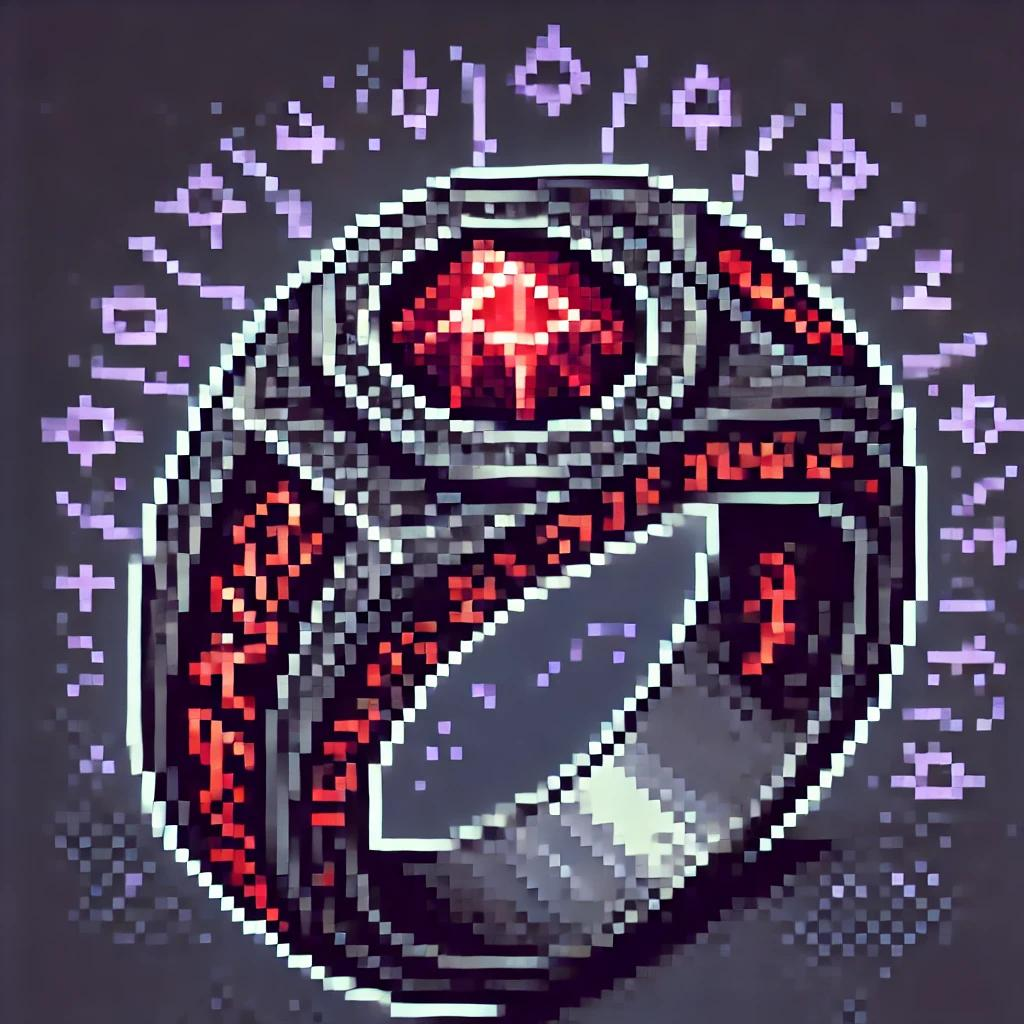
\includegraphics[height=4cm]{Bague du mage noir.jpg}
                    \caption{Bague du mage noir}
                    \label{fig:BagueMageNoir}
                \end{minipage}
                \hfill
                % Deuxième image
                \begin{minipage}{0.45\textwidth}
                    \centering
                    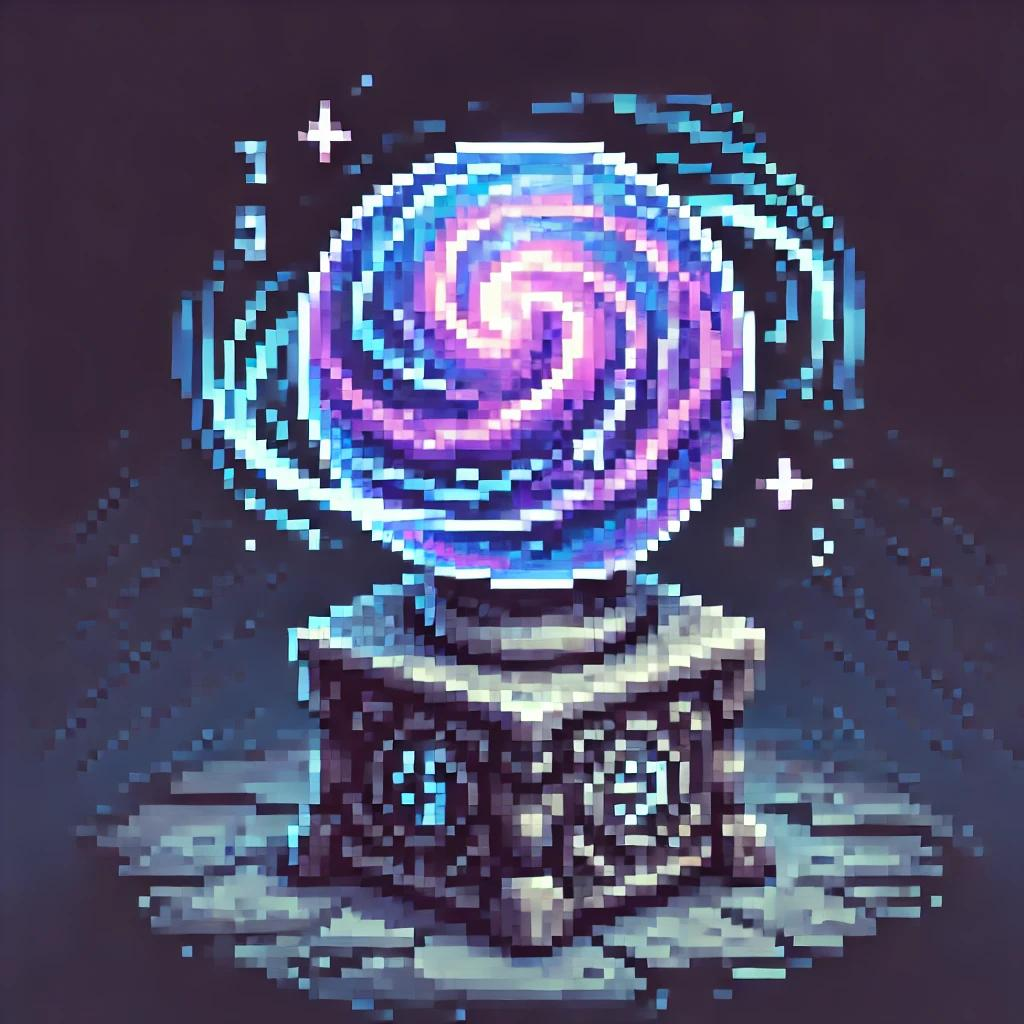
\includegraphics[height=4cm]{Orbe mystique.jpg}
                    \caption{Orbe mystique}
                    \label{fig:OrbeMystique}
                \end{minipage}
            \end{figure}
            \subsubsection{Sprites et Personnages}
            Il y a quatre personnages dans le jeu :
            \begin{itemize}
                \item Archer
                \item Mage
                \item Ninja
                \item Vampire
            \end{itemize}
            Chaque personnage à un spritesheet de 12 images (3 images par direction).\\
            Quelques exemples de spritesheet ci-dessous (Figure~\ref{fig:Mage}, Figure~\ref{fig:Archer}). 
            \begin{figure}[H]
                \centering
                % Première image
                \begin{minipage}{0.45\textwidth}
                    \centering
                    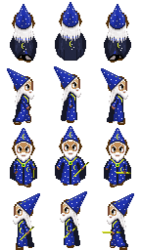
\includegraphics[height=4cm]{mageSrc.png}
                    \caption{spritesheet Mage}
                    \label{fig:Mage}
                \end{minipage}
                \hfill
                % Deuxième image
                \begin{minipage}{0.45\textwidth}
                    \centering
                    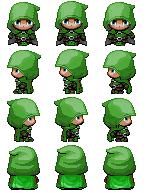
\includegraphics[height=4cm]{archerSRC.png}
                    \caption{spritesheet Archer}
                    \label{fig:Archer}
                \end{minipage}
            \end{figure}
            \subsubsection{Tuiles et Biomes}
            Il y a six biomes différents dans le jeu.\\
            Chaque biome a :
            \begin{itemize}
                \item une texture de base pour le sol (voir Figure~\ref{fig:normal})
                \item une texture pour un premier obstacle (voir Figure~\ref{fig:obstacle1})
                \item une texture pour un deuxième obstacle (voir Figure~\ref{fig:obstacle2})
                \item Une texture pour indiquer la sortie d'une tuile (voir Figure~\ref{fig:sortie})
            \end{itemize}
            Exemple des 4 textures du biome plaine ci-dessous. 
            \begin{figure}[H]
                \centering
                % Première image
                \begin{minipage}{0.45\textwidth}
                    \centering
                    
\includegraphics[height=1.5cm]{normal.png}
                    \caption{Texture base}
                    \label{fig:normal}
                \end{minipage}
                \hfill
                % Deuxième image
                \begin{minipage}{0.45\textwidth}
                    \centering
                    
\includegraphics[height=1.5cm]{obstacle1.png}
                    \caption{Texture obstacle1}
                    \label{fig:obstacle1}
                \end{minipage}
            \end{figure}
            \begin{figure}[H]
                \centering
                % Troisième image
                \begin{minipage}{0.45\textwidth}
                    \centering
                    
\includegraphics[height=1.5cm]{obstacle2.png}
                    \caption{Texture obstacle2}
                    \label{fig:obstacle2}
                \end{minipage}
                \hfill
                % Quatrième image
                \begin{minipage}{0.45\textwidth}
                    \centering
                    
\includegraphics[height=1.5cm]{sortie.png}
                    \caption{Texture sortie}
                    \label{fig:sortie}
                \end{minipage}
            \end{figure}

        \subsection{Implémentation}
        Nous allons maintenant présenter les différentes structures de données mises en œuvre qui représentent le jeu dans le programme.
            \subsubsection{Map}
            La map est inspirée des jeux comme \href{https://en.wikipedia.org/wiki/The_Binding_of_Isaac_(video_game)}{The Binding of Isaac}, 
            dans lesquels le joueur se déplace de salle en salle dans les quatre directions. \\
            On appelle ces salles des tuiles. De plus, la map est constituée de différents biomes qui déterminent l'apparence de la tuile. Similaires aux biomes de \href{https://fr.wikipedia.org/wiki/Minecraft}{Minecraft},
            les textures diffèrent selon les biomes (forêt, plaine, montagne, desert, neige, glace).
            Pour que le jeu soit re-jouable et intéressant, la map est générée procéduralement, en associant à chaque tuile un biome, 
            puis en créant les tuiles en plaçant les textures selon le biome choisi.\\
            Dans le programme écrit en C. La map est une matrice de tuile. Chaque tuile est une structure, qui contient l'information du biome, 
            une matrice des textures qui la composent et les éléments du jeu qui y sont associés.
            On représente les informations par des listes. Elles sont variables au cours du jeu et selon les tuiles. 
            Il y a quatre listes qui tiennent compte des joueurs, des objets, des monstres, et des effets des compétences actives afin de les afficher facilement.
            \subsubsection{Personnages}
            Les personnages sont choisis par les joueurs au début de la partie. Ils sont caractérisés par une classe, comme dans certains jeux de rôle. 
            Cette classe détermine les statistiques de base du personnage et les compétences accessibles. Les statistiques sont la vie, la force, la magie et la vitesse. 
            Chaque personnage a un point fort qui le distingue des autres.\\
            Le personnage est représenté par une structure C. Ses statistiques  sont deux tableaux de quatre valeurs, 
            une pour sauvegarder ses statistiques de base et l'autre pour avoir accès à ses statistiques améliorées par les objets. 
            Un tableau de pointeurs permet de retrouver les objets possédés par le joueur.\\
            La fonction creer\_perso permet d’initialiser un joueur à partir de la classe choisie.
            Celle pour détruire est appelée à la fin du programme.\\
            Pour gérer le déplacement des joueurs, on utilise SDL qui écoute les évènements du clavier. 
            En utilisant l’état des flèches directionnelles, on peut faire changer la direction du joueur avec changer\_dir. 
            Puis la fonction avancer est appelée et change la position du personnage graĉe à sa vitesse et sa direction en vérifiant qu’il ne dépasse pas les bords de la tuile. 
            Pour simplifier le calcul, on utilise une table de hachage qui donne une structure qui est le multiplicateur en x et en y selon la direction. \\\\
            \textit{
                Exemple : le joueur se déplace vers le haut et vers la droite, qui est converti en une valeur énumérée (type enum en C). \\
                Cette valeur donne un indice pour le tableau deplacement. La valeur qui correspond à cette direction est la structure de valeurs $x=1$ et $y=-1$, 
                car un déplacement vers la droite signifie ajouter une valeur x (la vitesse du joueur) 
                et un déplacement vers le haut implique de diminuer la valeur y du joueur de sa vitesse aussi.
            }
            \subsubsection{Compétences}
            Les compétences sont les capacités des personnages, elles peuvent être de simples attaques, des techniques de déplacement ou bien des sorts.
            \subsubsection{Objets}
            Les objets sont essentiels au jeu. Ils permettent d'augmenter les statisques de base de notre personnage. 
            Il y a 40 objets dans le jeu, séparés en 4 catégories de rareté : 
            \begin{itemize}
                \item commun
                \item rare
                \item épique
                \item légendaire
            \end{itemize}
            Chaque objet a 4 statisques différentes :
            \begin{itemize}
                \item vie
                \item force
                \item magie
                \item vitesse
            \end{itemize}
            Ensuite pour calculer le bonus apporté au joueur par chaque objet on différencie trois cas de figure :
            \begin{itemize}
                \item bonus nul
                \item bonus à additionner 
                \item bonus à multiplier
            \end{itemize}
            Pour garder une certaine cohérence dans les calculs de statisques du personnages un ordre de calcul a été décidé.
            On affectue d'abord les calculs de somme puis les calculs de produit. Pour ce faire chaque statisque de l'objet a un couple de valeur. 
            La première valeur corresponds à ce qui est a sommer ou multiplier à la statisque de base du personnage. 
            La deuxième valeur est un ordre de priorité permettant d'effectuer les calculs dans le bon ordre.
            \\
            \\
            \textit{
                Exemple : si un personnage a deux objets :
                \begin{itemize}
                    \item 1\textsuperscript{er} objet :\{\{0, null\}, \{10, add\}, \{0, null\}, \{-2, add\}\}
                    \item 2\textsuperscript{e} objet : \{\{1.5, mult\}, \{0.8, mult\}, \{20, add\}, \{0, null\}\}
                \end{itemize} 
                On rapelle que les statisques sont de la forme \{vie, force, magie, vitesse\}.
                Dans cet exemple, on commencera par calculer les trois additions puis les trois multiplications 
                (la somme étant représenté par «add» et le produit par «mult»).
            }\\\\
            Deux fonctions permettent de gérer les objets possédés par le joueur.
            La fonction ajouter\_objet permet de placer un nouvel objet dans l’inventaire à une place libre. La fonction retirer\_objet supprime l’objet à la position donnée.
            Ces fonctions sont appelées par des fonctions de plus haut niveau qui vérifient la présence d’un objet au sol et retirent ou ajoutent l’objet correspondant sur la tuile en fonction de l’action du joueur.

            La fonction update\_stats est appelée quand un joueur gagne ou perd un objet. Elle permet de recalculer les statistiques du personnage


            \subsubsection{Quêtes}
            \subsubsection{Monstres}
            Le jeu intègre des personnages non joueurs.
            Ce sont des monstres, appelés mobs. Lorsqu'il sont tués il permettent d'obtenir des objets qui augmentent les capacités de base de notre personnage.
            Les mobs ont plusieurs fonctionnalités. La première est qu'ils se rapprochent du joueur le plus proche à l'aide d'une fonction de calcul de distance.
            \\
            Une fois que cette distance est calculée, la direction que le mob doit prendre est choisie avec un calcul d'angle. 
            Un vecteur horizontal orienté à droite qui servira de base est créé ainsi qu'un vecteur représentant la direction personnage vers mobs. (Voir Figure~\ref{fig:Mob}) 
            On calcule l'angle en radians formé par ces deux vecteurs.
            On obtient donc une valeur du cercle trigonométrique que l'on exploite de la manière suivante : 
            \begin{itemize}
                \item Le monstre va en haut si   $ \frac{\pi}{4}  \leq \text{angle} < \frac{3\pi}{4} $
                \item Le monstre va a gauche si  $ \frac{3\pi}{4} \leq \text{angle} < \frac{5\pi}{4} $
                \item Le monstre va en bas si    $ \frac{5\pi}{4} \leq \text{angle} < \frac{7\pi}{4} $
                \item Le monstre va a droite si  $ \frac{-\pi}{4} \leq \text{angle} < \frac{\pi}{4} $
            \end{itemize}

            \begin{figure}[H]
                \centering
                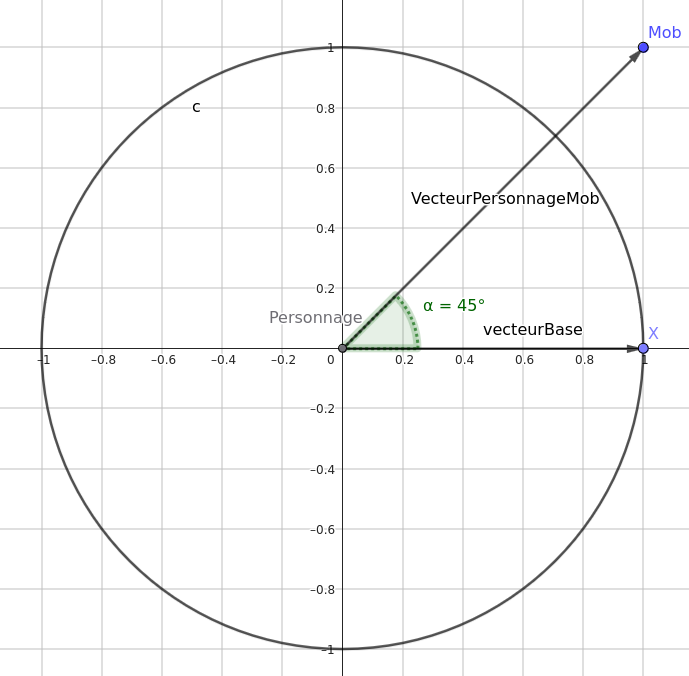
\includegraphics[height=9cm]{cercleTrigo.png}
                \caption{Représentation d'un calcul d'angle en fonction de la position d'un personnage et d'un mob}
                \label{fig:Mob}
            \end{figure}

            \subsubsection{Évènement}
        \subsection{Réseau}
        Nous allons maintenant voir comment connecter les joueurs avec un serveur pour permettre la connexion et le jeu.
	    Tout d’abord la communication à travers le réseau se fait par des écoutes et des envois dans différents flux. 
        Le client n’a donc comme flux, seulement le serveur. Le serveur a bien plus de flux, un pour chaque joueur. 
        La parallélisation est donc obligatoire.

            \subsubsection{Networking}
            Il y a tout d’abord une étape ou le client se connecte au serveur, suite au choix réalisé dans le menu et suite à la l’initialisation du serveur. 
            Plusieurs structures vont être créées et la parallélisation démarre.
            \\
            L’envoi et la réception de données s’assure avec deux fonctions principales :
            La fonction send (qui n’est pas bloquante) permet l’envoi d’un paquet en unicast.
            La fonction recv (qui est bloquante) permet l’écoute du flux et la réception des paquets.
            \\
            La propriété bloquante de recv force l’utilisation de threads.
            Ainsi dès la première connexion, une fonction parallèle d’écoute est créée.
            Le programme possède donc à ce moment :
            \begin{itemize}
                \item Le programme principal qui a appelé la création des autres threads.
                \item Un (ou plusieurs pour le serveur) thread(s) d’écoute. 
            \end{itemize}
            La connexion entre eux se fait par une file. Les threads d’écoute enfilent et le programme principal défile les informations envoyées par le serveur. 
            Ces informations passent ainsi du serveur à l’écoute au main pour ensuite être traitées. \\
            Cette file permet aussi au serveur de traiter les différents clients.\\\\
            Différents code peuvent être utilisé lors de l’envoi de paquets (Voir Table~\ref{tab:tabCliServ}): 
    
            \begin{table}[h]
                \centering
                \begin{tabular}{|c|c|c|}
                    \hline
                    Code & Nom & Catégorie \\
                    \hline
                    11 & JOUEUR\_CHANGE\_DIR & Joueur \\
                    12 & JOUEUR\_MV & Joueur \\
                    13 & JOUEUR\_MV\_TUILES & Joueur \\
                    ... & ... & ... \\
                    20 & ADD\_OBJET & Objet \\
                    21 & RM\_OBJET & Objet \\
                    ... & ... & ... \\
                    301 & UPDATE\_ZONE & Compétence de zone \\
                    302 & RM\_ZONE & Compétence de zone \\
                    ... & ... & ... \\
                    \hline
                \end{tabular}
                \caption{Différents codes d'action entre le client et le serveur}
                \label{tab:tabCliServ}
            \end{table}

            \subsubsection{Client}
            \subsubsection{Serveur}
        \subsection{Rendu Graphique}
        Cette partie traitera de l'utilisation de la librairie SDL2 qui sert pour le rendu graphique du jeu.
            \subsubsection{Menu Principal}
            \subsubsection{Jeu}
            Dans cette partie, nous présenterons les moyens d’affichage des différents composants du jeu.\\\\
            Dans le jeu, le rendu de la map est généré en plusieurs étapes. Premièrement, la fonction init\_biomes charge toutes les textures du jeu
            qui composent les tuiles. Ensuite, les fonctions init\_map et init\_tuile génèrent pour chaque tuile une instance d’un biome. Enfin, il reste la phase d’exploitation : 
            quand un joueur entre sur une tuile. La fonction charger\_tuile s’occupe de créer le rendu qui sera affiché sur l’écran (qui est fixe) 
            à partir de la matrice de la tuile.
            Dans la boucle du jeu, cette texture est affichée avant les autres éléments du jeu à l’écran, graĉe à la bibliothèque SDL, car elle est le décor.\\
            Pour l’affichage des personnages. Nous avons développé une fonction charger\_sdl\_joueurs, qui prend en paramètres le tableau des joueurs et un tableau 
            à deux dimensions qui stocke les différentes textures des personnages. La fonction s’occupe de charger les bonnes images en fonction de la classe de chaque joueur. 
            Dans la boucle principale du client, la liste des personnages présents est parcourue, on affiche alors la texture du personnage qui correspond à sa direction, 
            à sa position courante.\\
            L’affichage des objets est similaire, les textures sont préchargées, puis, graĉe à la liste qui tient compte de ceux qui sont présents sur la même tuile 
            que le joueur, ils sont affichés.\\
            Les fonctions de destruction et de libération des ressources sont appelées à la fin du programme. 
            Les textures des objets, personnages, biomes doivent être détruites par la fonction SDL adéquate. 
            Tous les éléments des listes de chaque tuile sont aussi supprimés par detruire\_tuile, faisant appel à detruire\_liste.

                
    \section{Résultats et conclusion}
    \section{Annexes}

\end{document}